% Archivo de caracterización de infraestructura corregido

% Torre HP 1
\begin{table}[H]
\centering
\caption{Ficha técnica --- Torre 1}\label{tab:torre-hp-1}
\begin{tabular}{|p{0.6\textwidth}|p{0.3\textwidth}|}
\hline
\multicolumn{2}{|l|}{\textbf{DESCRIPCIÓN FÍSICA:} Servidor tipo torre} \\ \hline
\textbf{TIPO DE RECURSO:} Torre &
\multirow{5}{*}{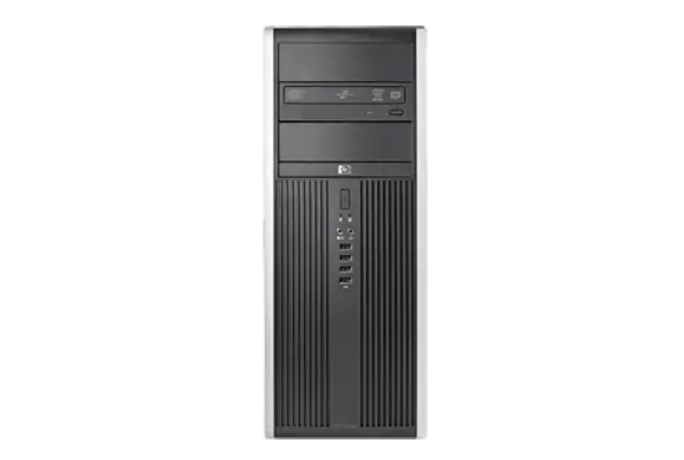
\includegraphics[width=0.25\textwidth,height=4cm,keepaspectratio]{tablas-images/cp1/torres/torre-1.png}} \\ \cline{1-1}
\textbf{MODELO:} Desconocido & \\ \cline{1-1}
\textbf{MARCA:} HP & \\ \cline{1-1}
\textbf{CÓDIGO DE INVENTARIO:} 7 24390 49867 3 & \\ \cline{1-1}
\textbf{NÚMERO EN CPD:} 14 & \\ \hline
\multicolumn{2}{|l|}{\textbf{ESPECIFICACIONES TÉCNICAS}} \\ \hline
\multicolumn{2}{|p{0.95\textwidth}|}{
\footnotesize
- 8 entradas USB (4 al frente, 4 en la parte trasera)
- Entrada de audio y microfono
- Entrada HDMI
- Lector de DVDs
- 3 puertos Ethernet (Parte trasera)
- Entrada Displayport
- Puertos PS/2 (Teclado y Ratón)
} \\ \hline
\multicolumn{2}{|l|}{\textbf{PROPÓSITO:} Hipervisor de XCP-ng} \\ \hline
\multicolumn{2}{|l|}{\textbf{OPORTUNIDAD DE USO:} Proyectos del \GRID} \\ \hline
\multicolumn{2}{|p{0.9\textwidth}|}{\textbf{OBSERVACIONES:} El Equipo no tiene modelo. El equipo está diseñado para usuario final pero fue adaptado para entornos de virtualización.} \\ \hline
\end{tabular}
\end{table}


% Torre 2
\begin{table}[H]
\centering
\caption{Ficha técnica --- Torre 2}\label{tab:torre-2}
\begin{tabular}{|p{0.6\textwidth}|p{0.3\textwidth}|}
\hline
\multicolumn{2}{|l|}{\textbf{DESCRIPCIÓN FÍSICA:} Servidor tipo torre} \\ \hline
\textbf{TIPO DE RECURSO:} Torre & 
\multirow{5}{*}{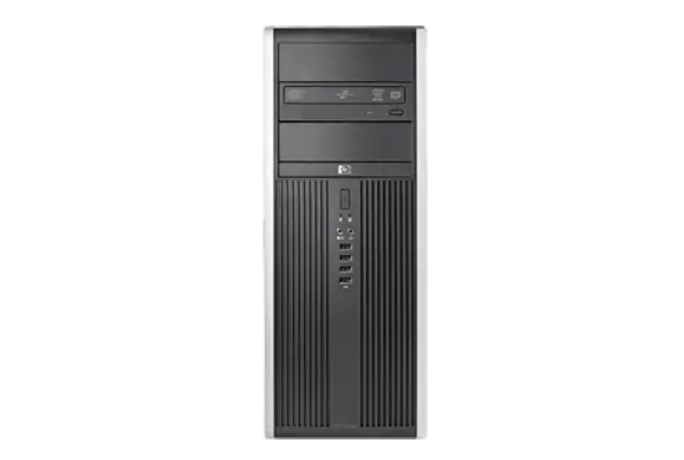
\includegraphics[width=0.25\textwidth,height=4cm,keepaspectratio]{tablas-images/cp1/torres/torre-1.png}} \\ \cline{1-1}
\textbf{MODELO:} Desconocido & \\ \cline{1-1}
\textbf{MARCA:} HP & \\ \cline{1-1}
\textbf{CÓDIGO DE INVENTARIO:} 7 24390 49861 1 & \\ \cline{1-1}
\textbf{NÚMERO EN CPD:} 12 & \\ \hline
\multicolumn{2}{|l|}{\textbf{ESPECIFICACIONES TÉCNICAS}} \\ \hline
\multicolumn{2}{|p{0.95\textwidth}|}{
\footnotesize
- 8 entradas USB (4 al frente, 4 en la parte trasera)
- Entrada de audio y microfono
- Entrada HDMI
- Lector de DVDs
- 3 puertos Ethernet (Parte trasera)
- Entrada Displayport
- Puertos PS/2 (Teclado y Ratón)
} \\ \hline
\multicolumn{2}{|l|}{\textbf{PROPÓSITO:} Hipervisor de XCP-ng} \\ \hline
\multicolumn{2}{|l|}{\textbf{OPORTUNIDAD DE USO:} Proyectos del \GRID} \\ \hline
\multicolumn{2}{|p{0.9\textwidth}|}{\textbf{OBSERVACIONES:} El Equipo no tiene modelo. El equipo está diseñado para usuario final pero fue adaptado para entornos de virtualización.} \\ \hline
\end{tabular}
\end{table}

% Torre 3
\begin{table}[H]
\centering
\caption{Ficha técnica -- Torre 3}
\label{tab:torre-3}
\begin{tabular}{|p{0.6\textwidth}|p{0.3\textwidth}|}
\hline
\multicolumn{2}{|l|}{\textbf{DESCRIPCIÓN FÍSICA:} Servidor tipo torre} \\ \hline
\textbf{TIPO DE RECURSO:} Torre & 
\multirow{5}{*}{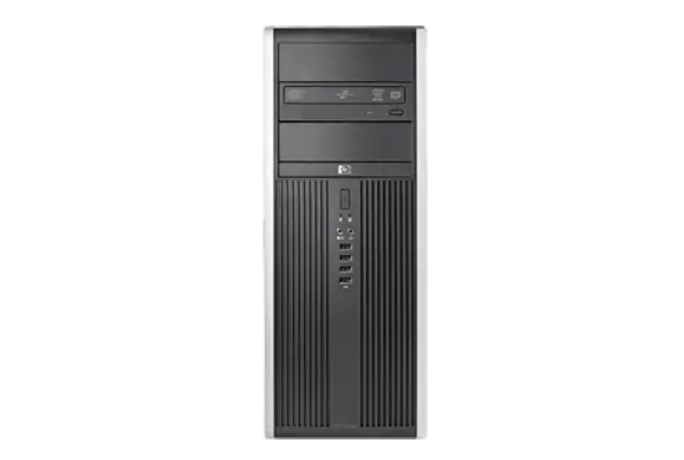
\includegraphics[width=0.25\textwidth,height=4cm,keepaspectratio]{tablas-images/cp1/torres/torre-1.png}} \\ \cline{1-1}
\textbf{MODELO:} Desconocido & \\ \cline{1-1}
\textbf{MARCA:} HP & \\ \cline{1-1}
\textbf{CÓDIGO DE INVENTARIO:} 7 24390 49969 4 & \\ \cline{1-1}
\textbf{NÚMERO EN CPD:} 13 & \\ \hline
\multicolumn{2}{|l|}{\textbf{ESPECIFICACIONES TÉCNICAS}} \\ \hline
\multicolumn{2}{|p{0.95\textwidth}|}{
\footnotesize
- 8 entradas USB (4 al frente, 4 en la parte trasera)
- Entrada de audio y microfono
- Entrada HDMI
- Lector de DVDs
- 3 puertos Ethernet (Parte trasera)
- Entrada Displayport
- Puertos PS/2 (Teclado y Ratón)
} \\ \hline
\multicolumn{2}{|l|}{\textbf{PROPÓSITO:} Hipervisor de XCP-ng} \\ \hline
\multicolumn{2}{|l|}{\textbf{OPORTUNIDAD DE USO:} Proyectos del \GRID} \\ \hline
\multicolumn{2}{|p{0.9\textwidth}|}{\textbf{OBSERVACIONES:} El Equipo no tiene modelo. El equipo está diseñado para usuario final pero fue adaptado para entornos de virtualización.} \\ \hline
\end{tabular}
\end{table}

% Torre 4
\begin{table}[H]
\centering
\caption{Ficha técnica --- Torre 4}
\label{tab:torre-4}
\begin{tabular}{|p{0.6\textwidth}|p{0.3\textwidth}|}
\hline
\multicolumn{2}{|l|}{\textbf{DESCRIPCIÓN FÍSICA:} Servidor tipo torre} \\ \hline
\textbf{TIPO DE RECURSO:} Torre & 
\multirow{5}{*}{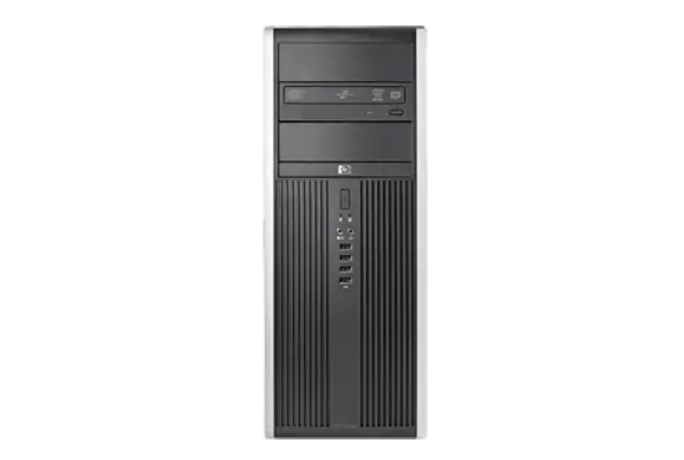
\includegraphics[width=0.25\textwidth,height=4cm,keepaspectratio]{tablas-images/cp1/torres/torre-1.png}} \\ \cline{1-1}
\textbf{MODELO:} Desconocido & \\ \cline{1-1}
\textbf{MARCA:} HP & \\ \cline{1-1}
\textbf{CÓDIGO DE INVENTARIO:} 7 24390 49879 4 & \\ \cline{1-1}
\textbf{NÚMERO EN CPD:} 14 & \\ \hline
\multicolumn{2}{|l|}{\textbf{ESPECIFICACIONES TÉCNICAS}} \\ \hline
\multicolumn{2}{|p{0.95\textwidth}|}{
\footnotesize
- 8 entradas USB (4 al frente, 4 en la parte trasera)
- Entrada de audio y microfono
- Entrada HDMI
- Lector de DVDs
- 3 puertos Ethernet (Parte trasera)
- Entrada Displayport
- Puertos PS/2 (Teclado y Ratón)
} \\ \hline
\multicolumn{2}{|l|}{\textbf{PROPÓSITO:} Hipervisor de XCP-ng} \\ \hline
\multicolumn{2}{|l|}{\textbf{OPORTUNIDAD DE USO:} Proyectos del \GRID} \\ \hline
\multicolumn{2}{|p{0.9\textwidth}|}{\textbf{OBSERVACIONES:} El Equipo no tiene modelo. El equipo está diseñado para usuario final pero fue adaptado para entornos de virtualización.} \\ \hline
\end{tabular}
\end{table}

% Torre 5
\begin{table}[H]
\centering
\caption{Ficha técnica --- Torre 5}
\label{tab:torre-5}
\begin{tabular}{|p{0.6\textwidth}|p{0.3\textwidth}|}
\hline
\multicolumn{2}{|l|}{\textbf{DESCRIPCIÓN FÍSICA:} Servidor tipo torre} \\ \hline
\textbf{TIPO DE RECURSO:} Torre & 
\multirow{5}{*}{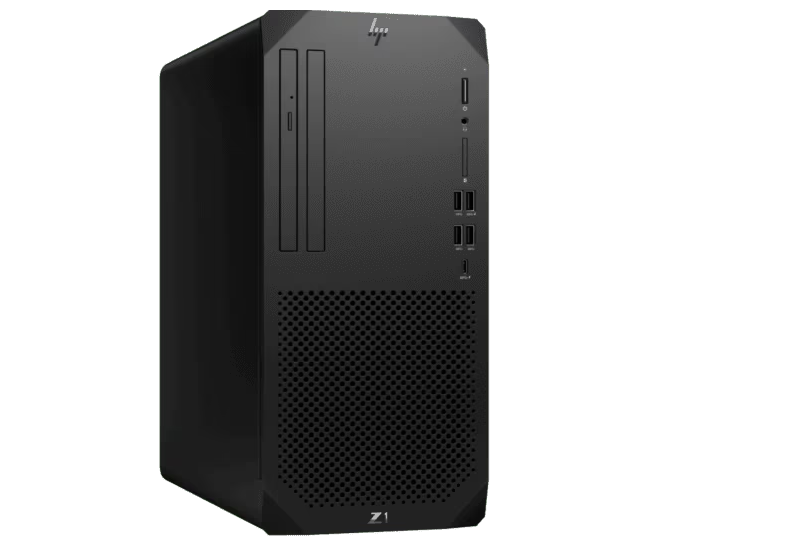
\includegraphics[width=0.25\textwidth,height=4cm,keepaspectratio]{tablas-images/cp1/torres/torre-2.png}} \\ \cline{1-1}
\textbf{MODELO:} G9 & \\ \cline{1-1}
\textbf{MARCA:} HP & \\ \cline{1-1}
\textbf{CÓDIGO DE INVENTARIO:} 72992 & \\ \cline{1-1}
\textbf{NÚMERO EN CPD:} 22 & \\ \hline
\multicolumn{2}{|l|}{\textbf{ESPECIFICACIONES TÉCNICAS}} \\ \hline
\multicolumn{2}{|p{0.95\textwidth}|}{
\footnotesize
- 9 entradas USB (4 al frente, 5 en la parte trasera)
- Entrada de audio y microfono
- Entrada HDMI
- Lector de DVDs
- 1 puerto Ethernet (Parte trasera)
- 2 Entrada Displayport
- Procesador Intel vPro i9
} \\ \hline
\multicolumn{2}{|l|}{\textbf{PROPÓSITO:} Hipervisor de XCP-ng} \\ \hline
\multicolumn{2}{|l|}{\textbf{OPORTUNIDAD DE USO:} Proyectos del \GRID} \\ \hline
\multicolumn{2}{|l|}{\textbf{OBSERVACIONES:} El equipo está diseñado para usuario final pero fue adaptado para entornos de virtualización.} \\ \hline
\end{tabular}
\end{table}

% Torre 6
\begin{table}[H]
\centering
\caption{Ficha técnica -- Torre 6}
\label{tab:torre-6}
\begin{tabular}{|p{0.6\textwidth}|p{0.3\textwidth}|}
\hline
\multicolumn{2}{|l|}{\textbf{DESCRIPCIÓN FÍSICA:} Servidor tipo torre} \\ \hline
\textbf{TIPO DE RECURSO:} Torre & 
\multirow{5}{*}{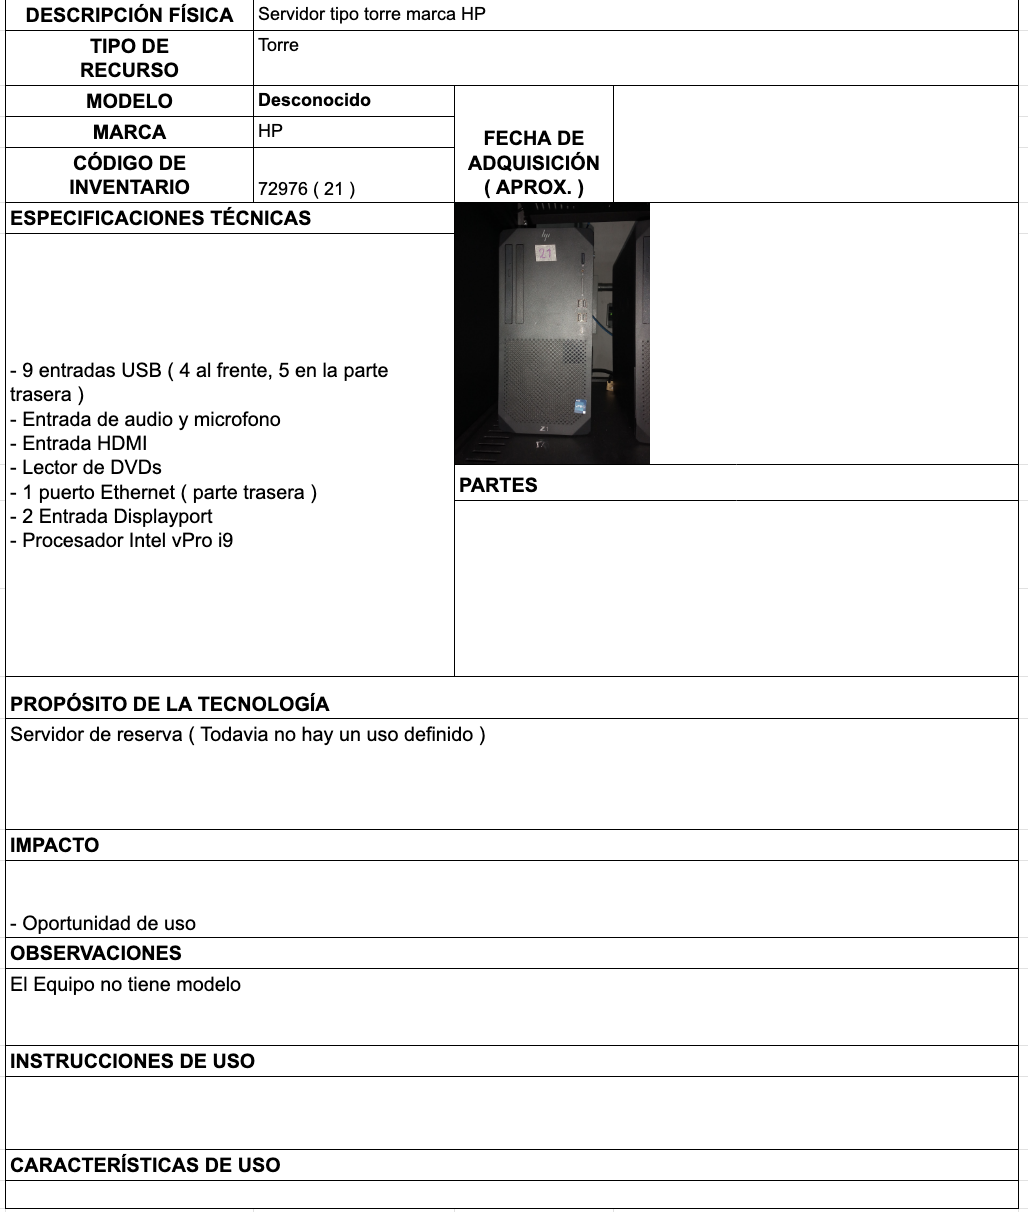
\includegraphics[width=0.25\textwidth,height=4cm,keepaspectratio]{tablas-images/cp1/torres/torre-6.png}} \\ \cline{1-1}
\textbf{MODELO:} Por definir & \\ \cline{1-1}
\textbf{MARCA:} Por definir & \\ \cline{1-1}
\textbf{CÓDIGO DE INVENTARIO:} Por definir & \\ \cline{1-1}
\textbf{FECHA DE ADQUISICIÓN (APROX.):} & \\ \hline
\multicolumn{2}{|l|}{\textbf{ESPECIFICACIONES TÉCNICAS}} \\ \hline
\multicolumn{2}{|p{0.95\textwidth}|}{
\footnotesize
Especificaciones por definir según imagen adjunta
} \\ \hline
\multicolumn{2}{|l|}{\textbf{PROPÓSITO:} Por definir} \\ \hline
\multicolumn{2}{|l|}{\textbf{IMPACTO:} Por evaluar} \\ \hline
\multicolumn{2}{|l|}{\textbf{OBSERVACIONES:} Ver imagen para detalles} \\ \hline
\end{tabular}
\end{table}

% Torre 7
\begin{table}[H]
\centering
\caption{Ficha técnica -- Torre 7}
\label{tab:torre-7}
\begin{tabular}{|p{0.6\textwidth}|p{0.3\textwidth}|}
\hline
\multicolumn{2}{|l|}{\textbf{DESCRIPCIÓN FÍSICA:} Servidor tipo torre} \\ \hline
\textbf{TIPO DE RECURSO:} Torre & 
\multirow{5}{*}{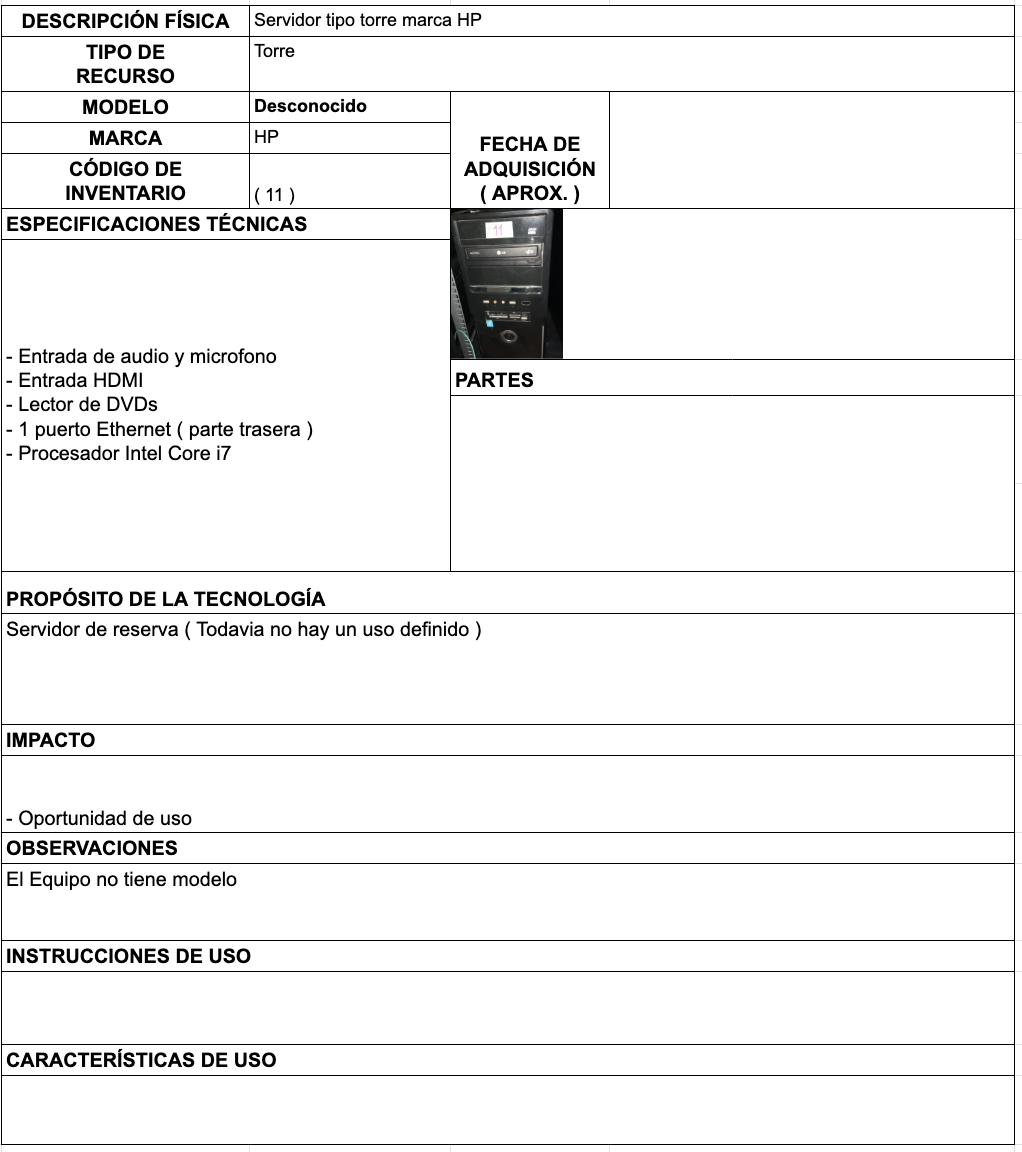
\includegraphics[width=0.25\textwidth,height=4cm,keepaspectratio]{tablas-images/cp1/torres/torre-7.png}} \\ \cline{1-1}
\textbf{MODELO:} Por definir & \\ \cline{1-1}
\textbf{MARCA:} Por definir & \\ \cline{1-1}
\textbf{CÓDIGO DE INVENTARIO:} Por definir & \\ \cline{1-1}
\textbf{FECHA DE ADQUISICIÓN (APROX.):} & \\ \hline
\multicolumn{2}{|l|}{\textbf{ESPECIFICACIONES TÉCNICAS}} \\ \hline
\multicolumn{2}{|p{0.95\textwidth}|}{
\footnotesize
Especificaciones por definir según imagen adjunta
} \\ \hline
\multicolumn{2}{|l|}{\textbf{PROPÓSITO:} Por definir} \\ \hline
\multicolumn{2}{|l|}{\textbf{IMPACTO:} Por evaluar} \\ \hline
\multicolumn{2}{|l|}{\textbf{OBSERVACIONES:} Ver imagen para detalles} \\ \hline
\end{tabular}
\end{table}

% Rack 1
\begin{table}[H]
\centering
\caption{Ficha técnica -- Rack 1}
\label{tab:rack-1}
\begin{tabular}{|p{0.6\textwidth}|p{0.3\textwidth}|}
\hline
\multicolumn{2}{|l|}{\textbf{DESCRIPCIÓN FÍSICA:} Servidor tipo rack} \\ \hline
\textbf{TIPO DE RECURSO:} Rack & 
\multirow{5}{*}{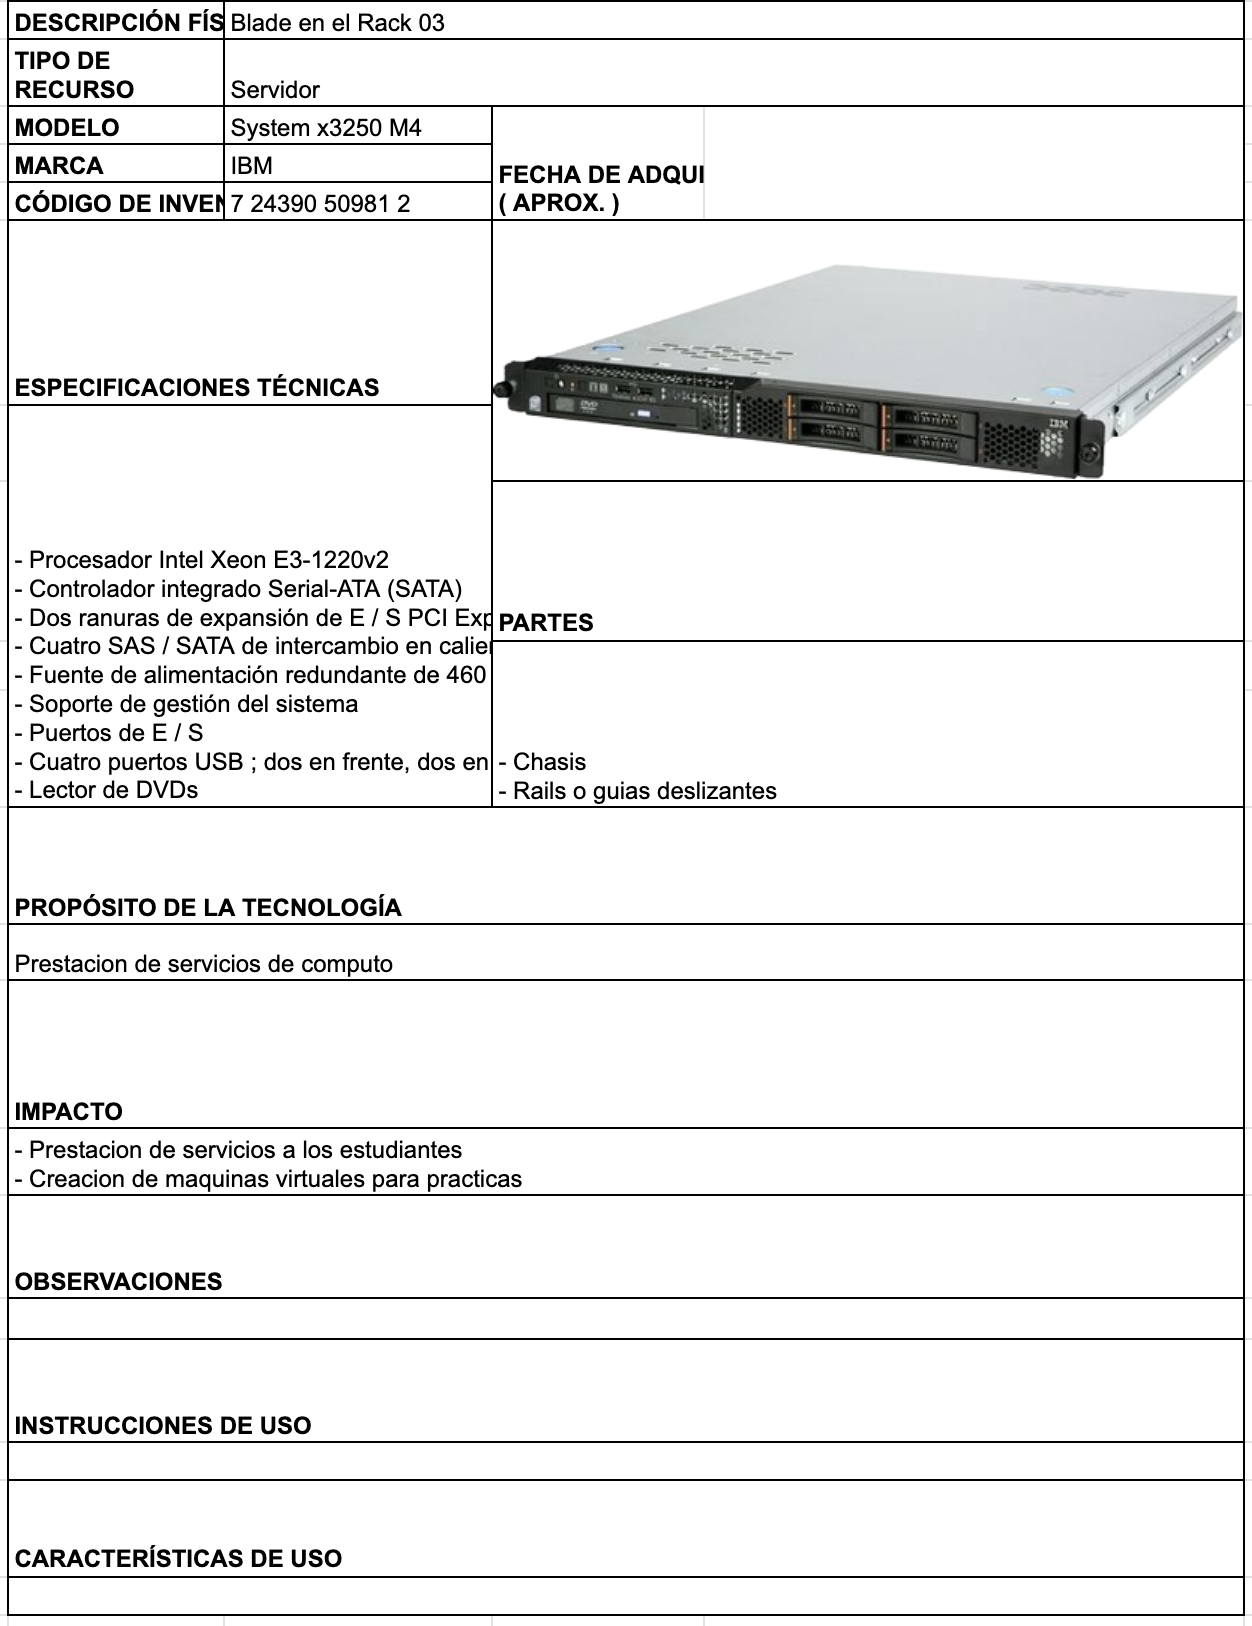
\includegraphics[width=0.25\textwidth,height=4cm,keepaspectratio]{tablas-images/cp1/racks/rack-1.png}} \\ \cline{1-1}
\textbf{MODELO:} Por definir & \\ \cline{1-1}
\textbf{MARCA:} Por definir & \\ \cline{1-1}
\textbf{CÓDIGO DE INVENTARIO:} Por definir & \\ \cline{1-1}
\textbf{FECHA DE ADQUISICIÓN (APROX.):} & \\ \hline
\multicolumn{2}{|l|}{\textbf{ESPECIFICACIONES TÉCNICAS}} \\ \hline
\multicolumn{2}{|p{0.95\textwidth}|}{
\footnotesize
Especificaciones por definir según imagen adjunta
} \\ \hline
\multicolumn{2}{|l|}{\textbf{PROPÓSITO:} Por definir} \\ \hline
\multicolumn{2}{|l|}{\textbf{IMPACTO:} Por evaluar} \\ \hline
\multicolumn{2}{|l|}{\textbf{OBSERVACIONES:} Ver imagen para detalles} \\ \hline
\end{tabular}
\end{table}

% Rack 2
\begin{table}[H]
\centering
\caption{Ficha técnica -- Rack 2}
\label{tab:rack-2}
\begin{tabular}{|p{0.6\textwidth}|p{0.3\textwidth}|}
\hline
\multicolumn{2}{|l|}{\textbf{DESCRIPCIÓN FÍSICA:} Servidor tipo rack} \\ \hline
\textbf{TIPO DE RECURSO:} Rack & 
\multirow{5}{*}{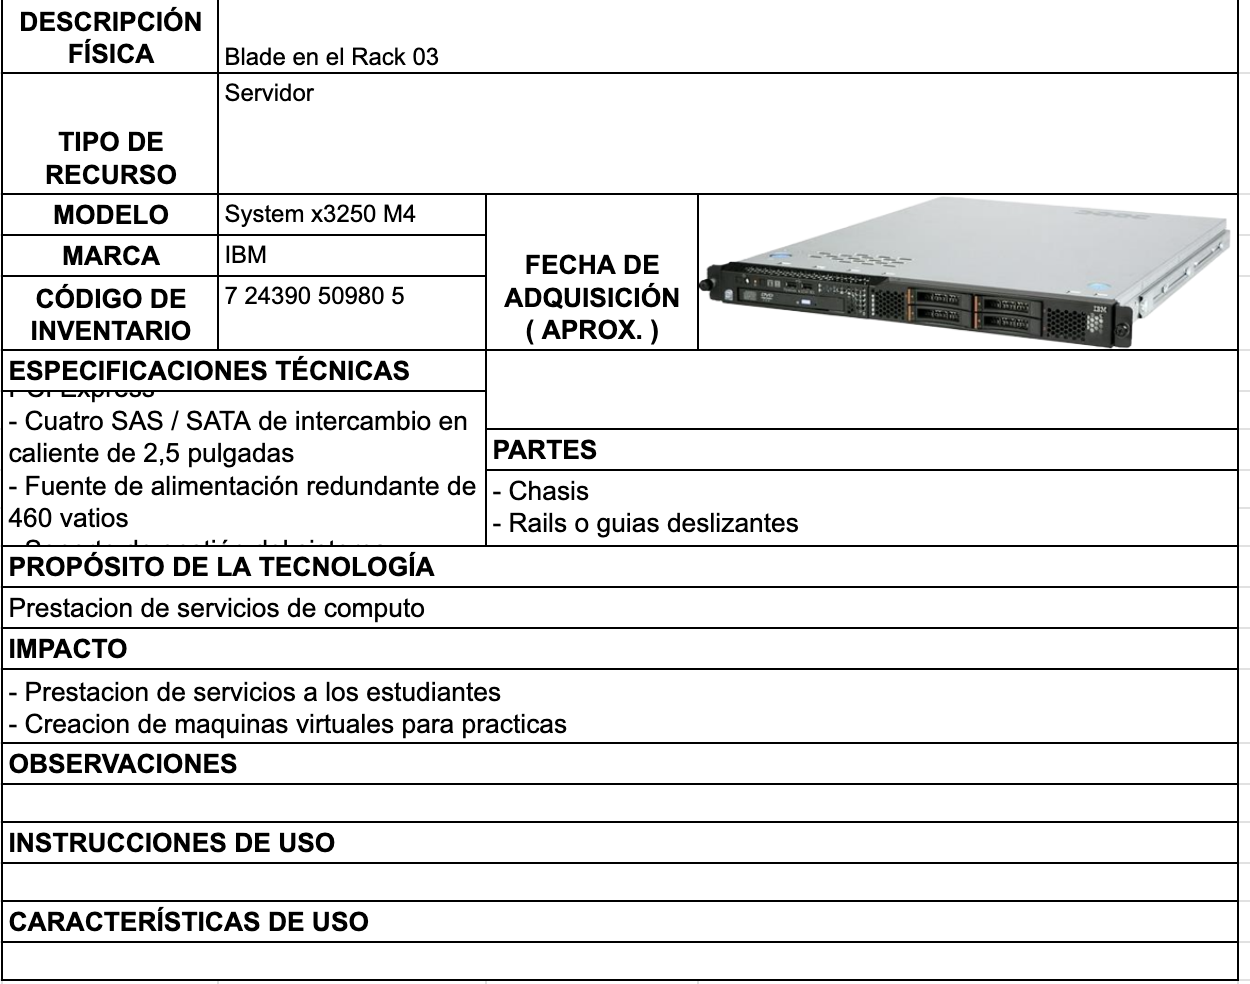
\includegraphics[width=0.25\textwidth,height=4cm,keepaspectratio]{tablas-images/cp1/racks/rack-2.png}} \\ \cline{1-1}
\textbf{MODELO:} Por definir & \\ \cline{1-1}
\textbf{MARCA:} Por definir & \\ \cline{1-1}
\textbf{CÓDIGO DE INVENTARIO:} Por definir & \\ \cline{1-1}
\textbf{FECHA DE ADQUISICIÓN (APROX.):} & \\ \hline
\multicolumn{2}{|l|}{\textbf{ESPECIFICACIONES TÉCNICAS}} \\ \hline
\multicolumn{2}{|p{0.95\textwidth}|}{
\footnotesize
Especificaciones por definir según imagen adjunta
} \\ \hline
\multicolumn{2}{|l|}{\textbf{PROPÓSITO:} Por definir} \\ \hline
\multicolumn{2}{|l|}{\textbf{IMPACTO:} Por evaluar} \\ \hline
\multicolumn{2}{|l|}{\textbf{OBSERVACIONES:} Ver imagen para detalles} \\ \hline
\end{tabular}
\end{table}

% Rack 3
\begin{table}[H]
\centering
\caption{Ficha técnica -- Rack 3}
\label{tab:rack-3}
\begin{tabular}{|p{0.6\textwidth}|p{0.3\textwidth}|}
\hline
\multicolumn{2}{|l|}{\textbf{DESCRIPCIÓN FÍSICA:} Servidor tipo rack} \\ \hline
\textbf{TIPO DE RECURSO:} Rack & 
\multirow{5}{*}{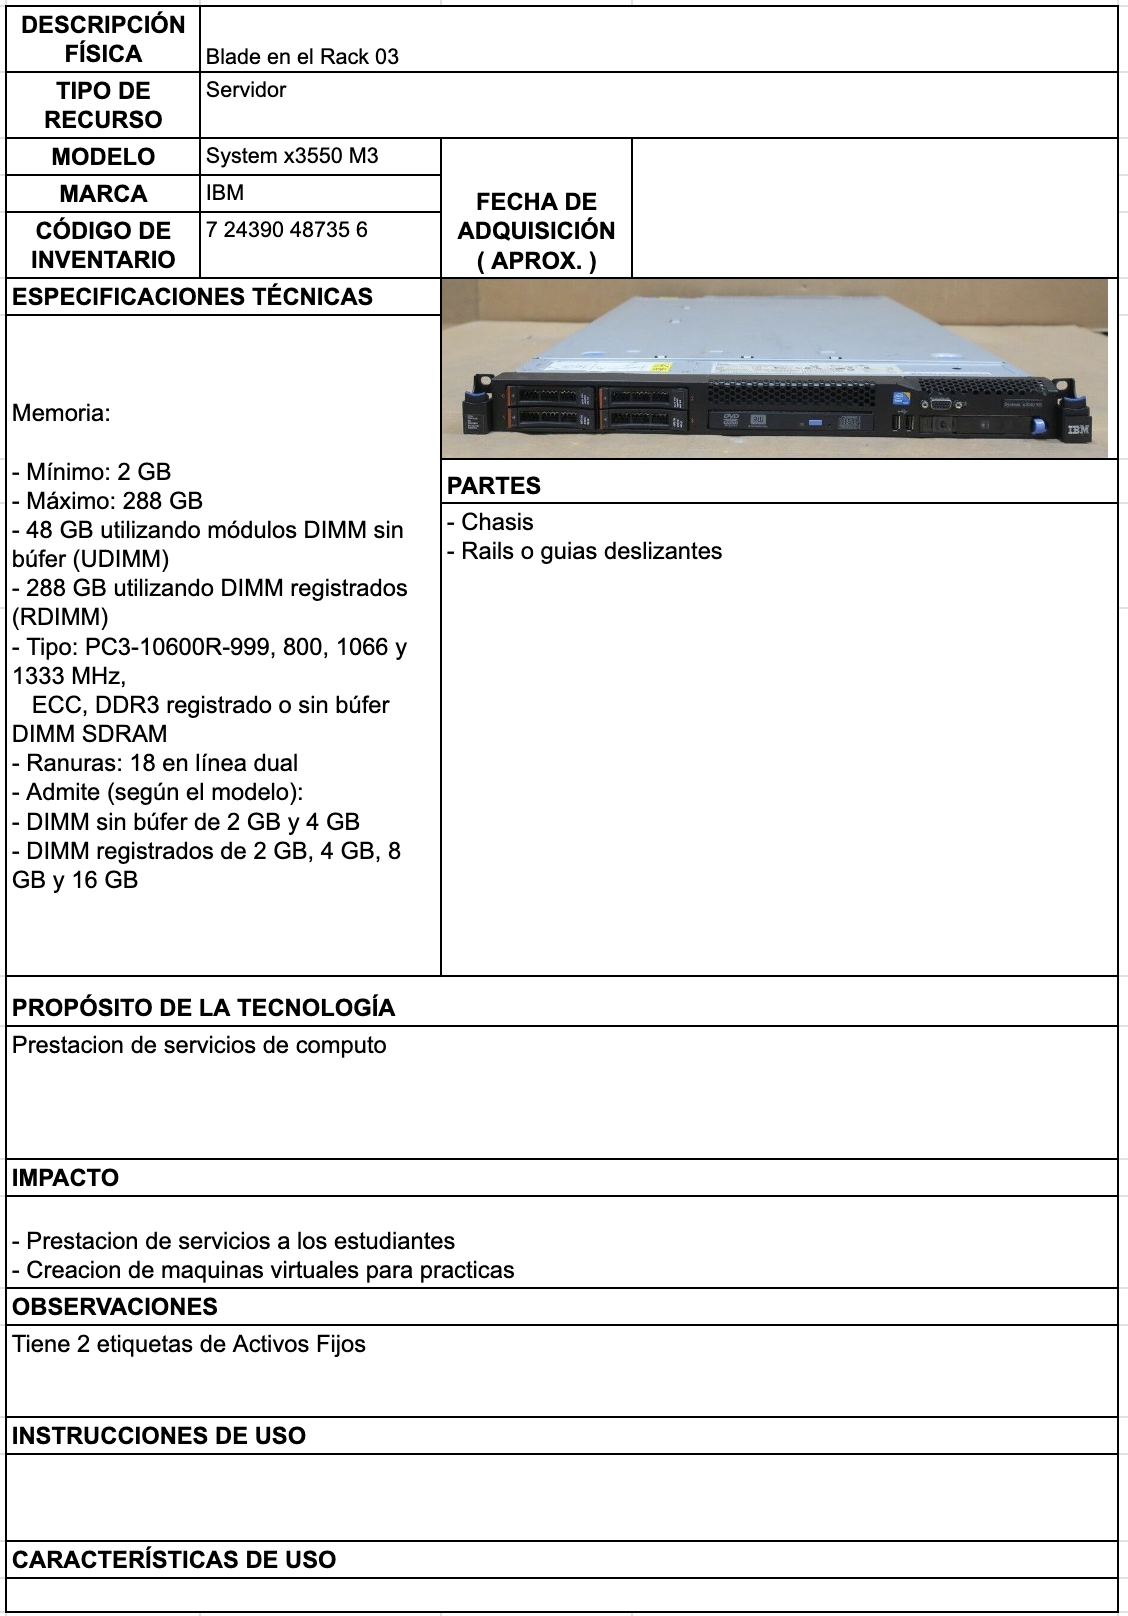
\includegraphics[width=0.25\textwidth,height=4cm,keepaspectratio]{tablas-images/cp1/racks/rack-3.png}} \\ \cline{1-1}
\textbf{MODELO:} Por definir & \\ \cline{1-1}
\textbf{MARCA:} Por definir & \\ \cline{1-1}
\textbf{CÓDIGO DE INVENTARIO:} Por definir & \\ \cline{1-1}
\textbf{FECHA DE ADQUISICIÓN (APROX.):} & \\ \hline
\multicolumn{2}{|l|}{\textbf{ESPECIFICACIONES TÉCNICAS}} \\ \hline
\multicolumn{2}{|p{0.95\textwidth}|}{
\footnotesize
Especificaciones por definir según imagen adjunta
} \\ \hline
\multicolumn{2}{|l|}{\textbf{PROPÓSITO:} Por definir} \\ \hline
\multicolumn{2}{|l|}{\textbf{IMPACTO:} Por evaluar} \\ \hline
\multicolumn{2}{|l|}{\textbf{OBSERVACIONES:} Ver imagen para detalles} \\ \hline
\end{tabular}
\end{table}

% Rack 4
\begin{table}[H]
\centering
\caption{Ficha técnica -- Rack 4}
\label{tab:rack-4}
\begin{tabular}{|p{0.6\textwidth}|p{0.3\textwidth}|}
\hline
\multicolumn{2}{|l|}{\textbf{DESCRIPCIÓN FÍSICA:} Servidor tipo rack} \\ \hline
\textbf{TIPO DE RECURSO:} Rack & 
\multirow{5}{*}{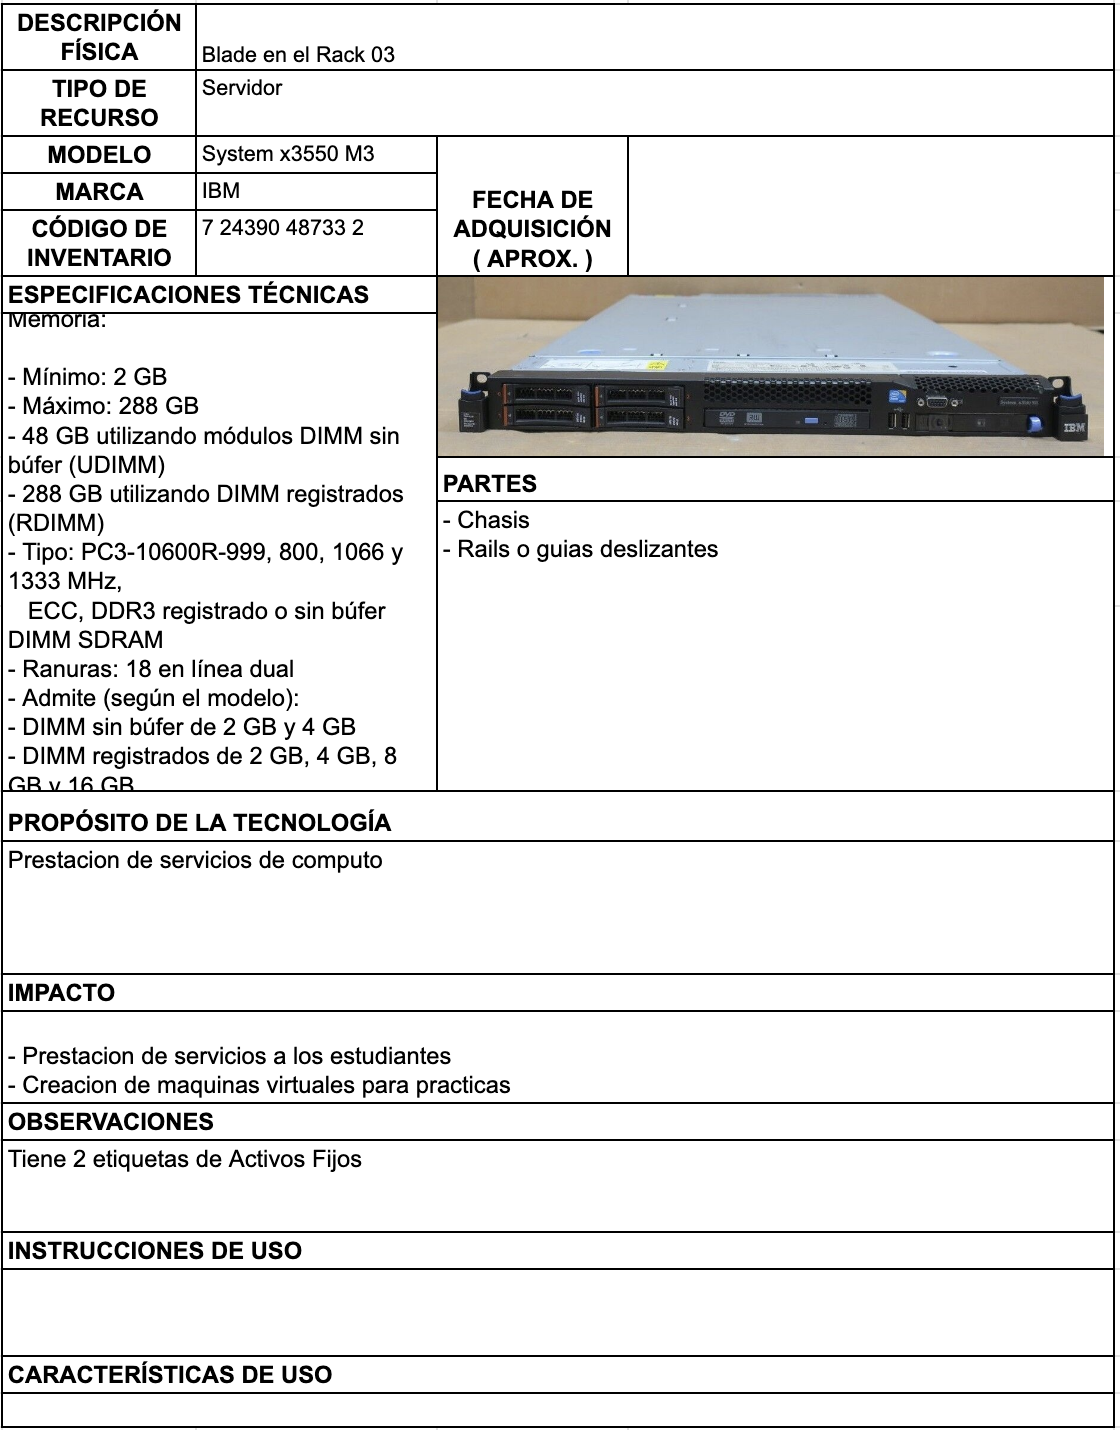
\includegraphics[width=0.25\textwidth,height=4cm,keepaspectratio]{tablas-images/cp1/racks/rack-4.png}} \\ \cline{1-1}
\textbf{MODELO:} Por definir & \\ \cline{1-1}
\textbf{MARCA:} Por definir & \\ \cline{1-1}
\textbf{CÓDIGO DE INVENTARIO:} Por definir & \\ \cline{1-1}
\textbf{FECHA DE ADQUISICIÓN (APROX.):} & \\ \hline
\multicolumn{2}{|l|}{\textbf{ESPECIFICACIONES TÉCNICAS}} \\ \hline
\multicolumn{2}{|p{0.95\textwidth}|}{
\footnotesize
Especificaciones por definir según imagen adjunta
} \\ \hline
\multicolumn{2}{|l|}{\textbf{PROPÓSITO:} Por definir} \\ \hline
\multicolumn{2}{|l|}{\textbf{IMPACTO:} Por evaluar} \\ \hline
\multicolumn{2}{|l|}{\textbf{OBSERVACIONES:} Ver imagen para detalles} \\ \hline
\end{tabular}
\end{table}

% Rack 5
\begin{table}[H]
\centering
\caption{Ficha técnica -- Rack 5}
\label{tab:rack-5}
\begin{tabular}{|p{0.6\textwidth}|p{0.3\textwidth}|}
\hline
\multicolumn{2}{|l|}{\textbf{DESCRIPCIÓN FÍSICA:} Servidor tipo rack} \\ \hline
\textbf{TIPO DE RECURSO:} Rack & 
\multirow{5}{*}{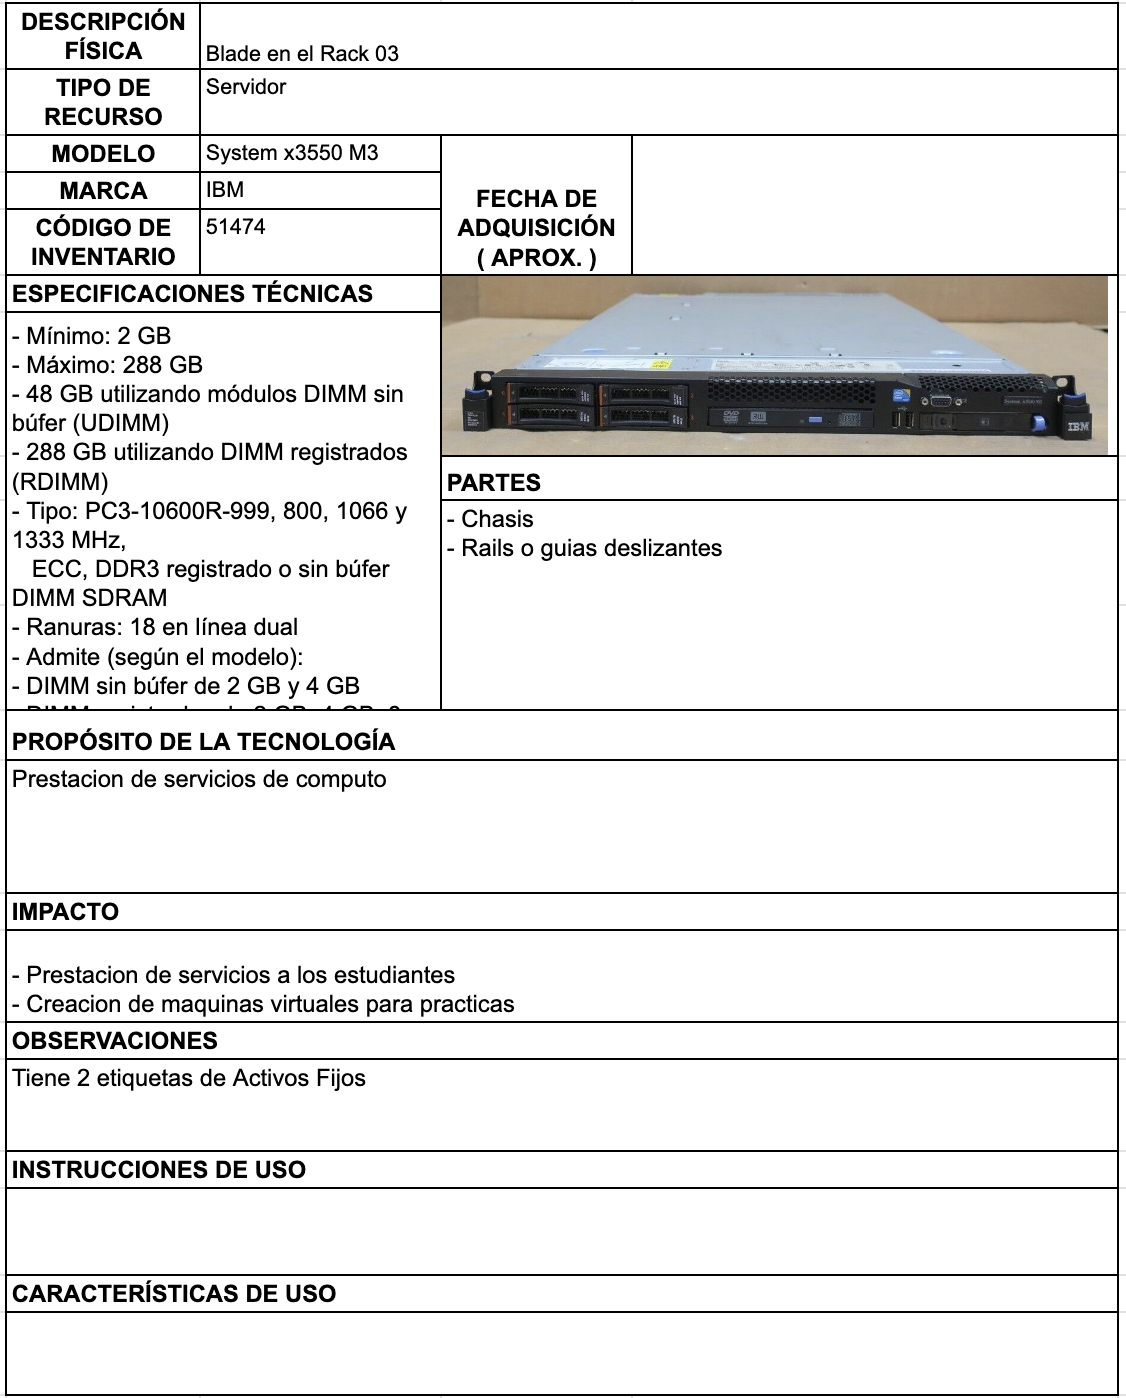
\includegraphics[width=0.25\textwidth,height=4cm,keepaspectratio]{tablas-images/cp1/racks/rack-5.png}} \\ \cline{1-1}
\textbf{MODELO:} Por definir & \\ \cline{1-1}
\textbf{MARCA:} Por definir & \\ \cline{1-1}
\textbf{CÓDIGO DE INVENTARIO:} Por definir & \\ \cline{1-1}
\textbf{FECHA DE ADQUISICIÓN (APROX.):} & \\ \hline
\multicolumn{2}{|l|}{\textbf{ESPECIFICACIONES TÉCNICAS}} \\ \hline
\multicolumn{2}{|p{0.95\textwidth}|}{
\footnotesize
Especificaciones por definir según imagen adjunta
} \\ \hline
\multicolumn{2}{|l|}{\textbf{PROPÓSITO:} Por definir} \\ \hline
\multicolumn{2}{|l|}{\textbf{IMPACTO:} Por evaluar} \\ \hline
\multicolumn{2}{|l|}{\textbf{OBSERVACIONES:} Ver imagen para detalles} \\ \hline
\end{tabular}
\end{table}

% NAS 1
\begin{table}[H]
\centering
\caption{Ficha técnica -- NAS 1}
\label{tab:nas-1}
\begin{tabular}{|p{0.6\textwidth}|p{0.3\textwidth}|}
\hline
\multicolumn{2}{|l|}{\textbf{DESCRIPCIÓN FÍSICA:} Sistema de almacenamiento conectado en red} \\ \hline
\textbf{TIPO DE RECURSO:} NAS (Network Attached Storage) & 
\multirow{5}{*}{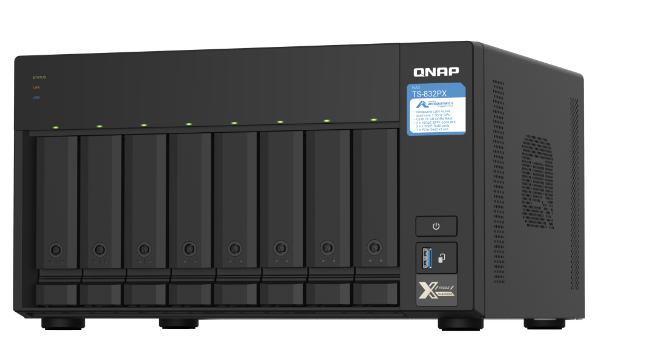
\includegraphics[width=0.25\textwidth,height=4cm,keepaspectratio]{tablas-images/cp1/NAS/nas-1.png}} \\ \cline{1-1}
\textbf{MODELO:} Por definir & \\ \cline{1-1}
\textbf{MARCA:} Por definir & \\ \cline{1-1}
\textbf{CÓDIGO DE INVENTARIO:} Por definir & \\ \cline{1-1}
\textbf{FECHA DE ADQUISICIÓN (APROX.):} & \\ \hline
\multicolumn{2}{|l|}{\textbf{ESPECIFICACIONES TÉCNICAS}} \\ \hline
\multicolumn{2}{|p{0.95\textwidth}|}{
\footnotesize
Especificaciones por definir según imagen adjunta
} \\ \hline
\multicolumn{2}{|l|}{\textbf{PROPÓSITO:} Por definir} \\ \hline
\multicolumn{2}{|l|}{\textbf{IMPACTO:} Por evaluar} \\ \hline
\multicolumn{2}{|l|}{\textbf{OBSERVACIONES:} Ver imagen para detalles} \\ \hline
\end{tabular}
\end{table}

% Firewall 1
\begin{table}[H]
\centering
\caption{Ficha técnica -- Firewall 1}
\label{tab:firewall-1}
\begin{tabular}{|p{0.6\textwidth}|p{0.3\textwidth}|}
\hline
\multicolumn{2}{|l|}{\textbf{DESCRIPCIÓN FÍSICA:} Sistema de seguridad de red} \\ \hline
\textbf{TIPO DE RECURSO:} Firewall & 
\multirow{5}{*}{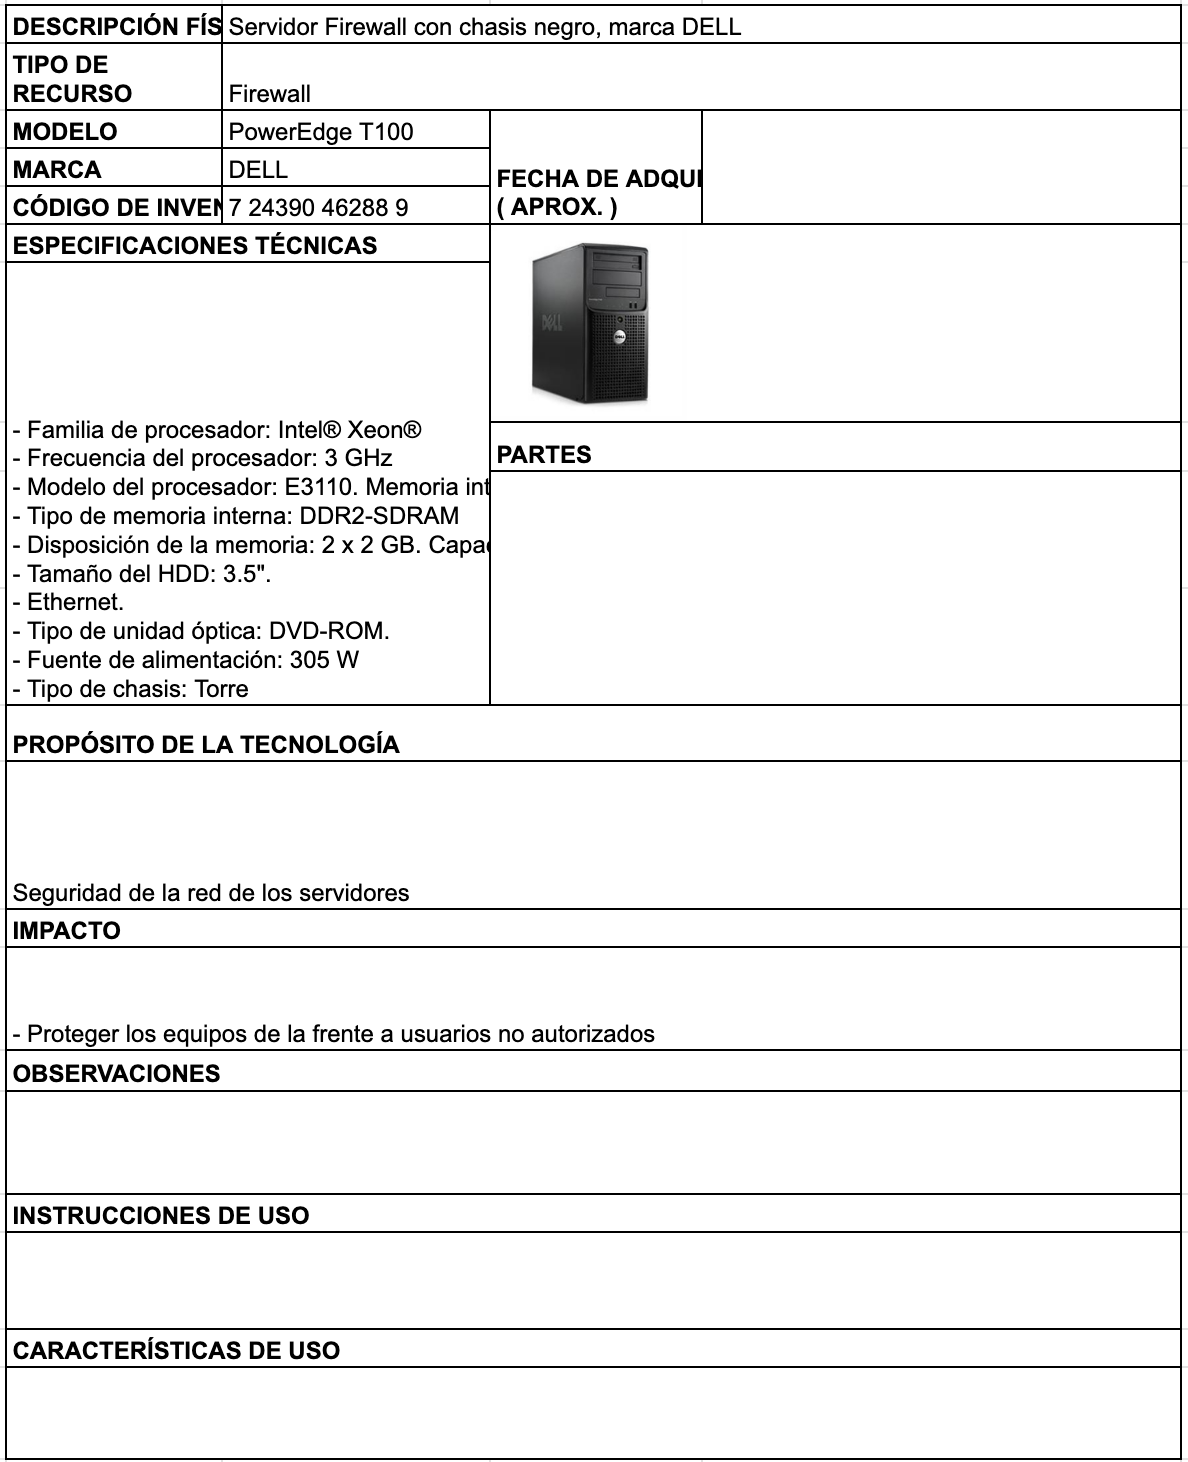
\includegraphics[width=0.25\textwidth,height=4cm,keepaspectratio]{tablas-images/cp1/firewall/firewall.png}} \\ \cline{1-1}
\textbf{MODELO:} Por definir & \\ \cline{1-1}
\textbf{MARCA:} Por definir & \\ \cline{1-1}
\textbf{CÓDIGO DE INVENTARIO:} Por definir & \\ \cline{1-1}
\textbf{FECHA DE ADQUISICIÓN (APROX.):} & \\ \hline
\multicolumn{2}{|l|}{\textbf{ESPECIFICACIONES TÉCNICAS}} \\ \hline
\multicolumn{2}{|p{0.95\textwidth}|}{
\footnotesize
Especificaciones por definir según imagen adjunta
} \\ \hline
\multicolumn{2}{|l|}{\textbf{PROPÓSITO:} Por definir} \\ \hline
\multicolumn{2}{|l|}{\textbf{IMPACTO:} Por evaluar} \\ \hline
\multicolumn{2}{|l|}{\textbf{OBSERVACIONES:} Ver imagen para detalles} \\ \hline
\end{tabular}
\end{table}